The main idea of logistic regression is to predict from a set of discrete binary values (ex: have cancer or not [0, 1]). In order to acomplish that, we use a linear function (Decision boundary, can be non-linear) to map all predictions greater than 0.5 as 1 and all less than 0.5 as a 0. This \textbf{prediction} is done by a \textbf{sigmoid} ($g(x)$) function that normalizes the output of the \textbf{Decision boundary} ($\theta^Tx$) to just 1 or 0.

So in conclusion, there is a \textbf{hypotheses} ($h_{\theta}(x)$) function that is the sigmoid ($g(x)$) function applied to the Decision boundary; and the \textbf{goal} is to find the most accurate parameters for the Decision boundary ($\theta^Tx$).

\subsection{Concepts}
\subsubsection{Sigmoid function}
Also called \textit{Logistic function}, maps any real number to the (0, 1) interval, making it useful for transforming an arbitrary-valued function into a function better suited for classification. The function has this form:

\begin{align}
	g(z) & = \frac{1}{1 + e^{-z}}
\end{align}

And looks like:
\begin{figure}[h]
    \centering
    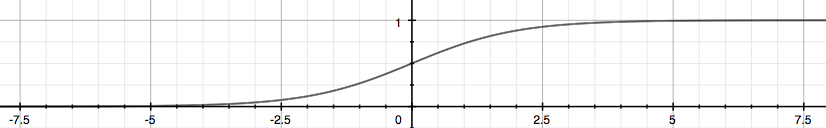
\includegraphics[width=1\textwidth]{sigmoid-function}
    \caption{Sigmoid function}
    \label{fig:sigmoid}
\end{figure}

\subsubsection{Hypotheses function}
This hypotheses function will predict, using some input data ($x_i$) and a set of precomputed coefficients ($\theta$), a number between 0 and 1.

$$0 \le h_{\theta}(x) \le 1$$

In order to achieve this, we use the sigmoid function to map our output to 0 - 1 interval on the decision boundary. The function has this form:

\begin{align}
	h_{\theta}(x) & = g(\theta^Tx) = g(X\theta)
\end{align}

$$h_{\theta}(x) = \frac{1}{1 + e^{-\theta^Tx}}$$

The result of this function can be interpreted as \textit{the probability that the output is 1}. For example, $h_{\theta}(x)=0.7$ gives us a probability of 70\% that our output is 1. Our probability that our prediction is 0 is just the complement of our probability that it is 1 (e.g. if probability that it is 1 is 70\%, then the probability that it is 0 is 30\%).


\subsubsection{Decision boundary}
This function describes the line (can be polynomial) that determines the limit of the features in order to predict whether 0 or 1. The representation for the decision boundary is:

$$\theta^Tx$$


\noindent In order to visualize it, we need to separate the ones that are $y = 0$ and the ones that are $y = 1$, then plot all features. But all axis must be the features ($x^{(j)}$) displayed separately the \textit{0's} from the \textit{1's}


\noindent And it can have many forms, also polynomial.


\begin{figure}[h]
	\begin{multicols}{2}
	\centering
	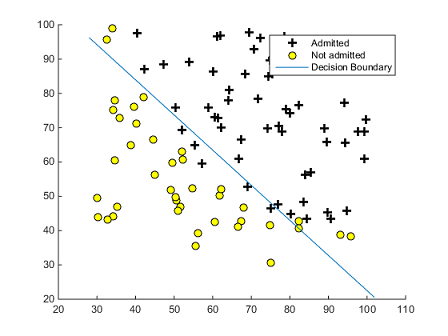
\includegraphics[width=0.4\textwidth]{decision-boundary}
	\caption{Linear Decision boundary}
	\label{fig:decision-boundary}

	\centering
	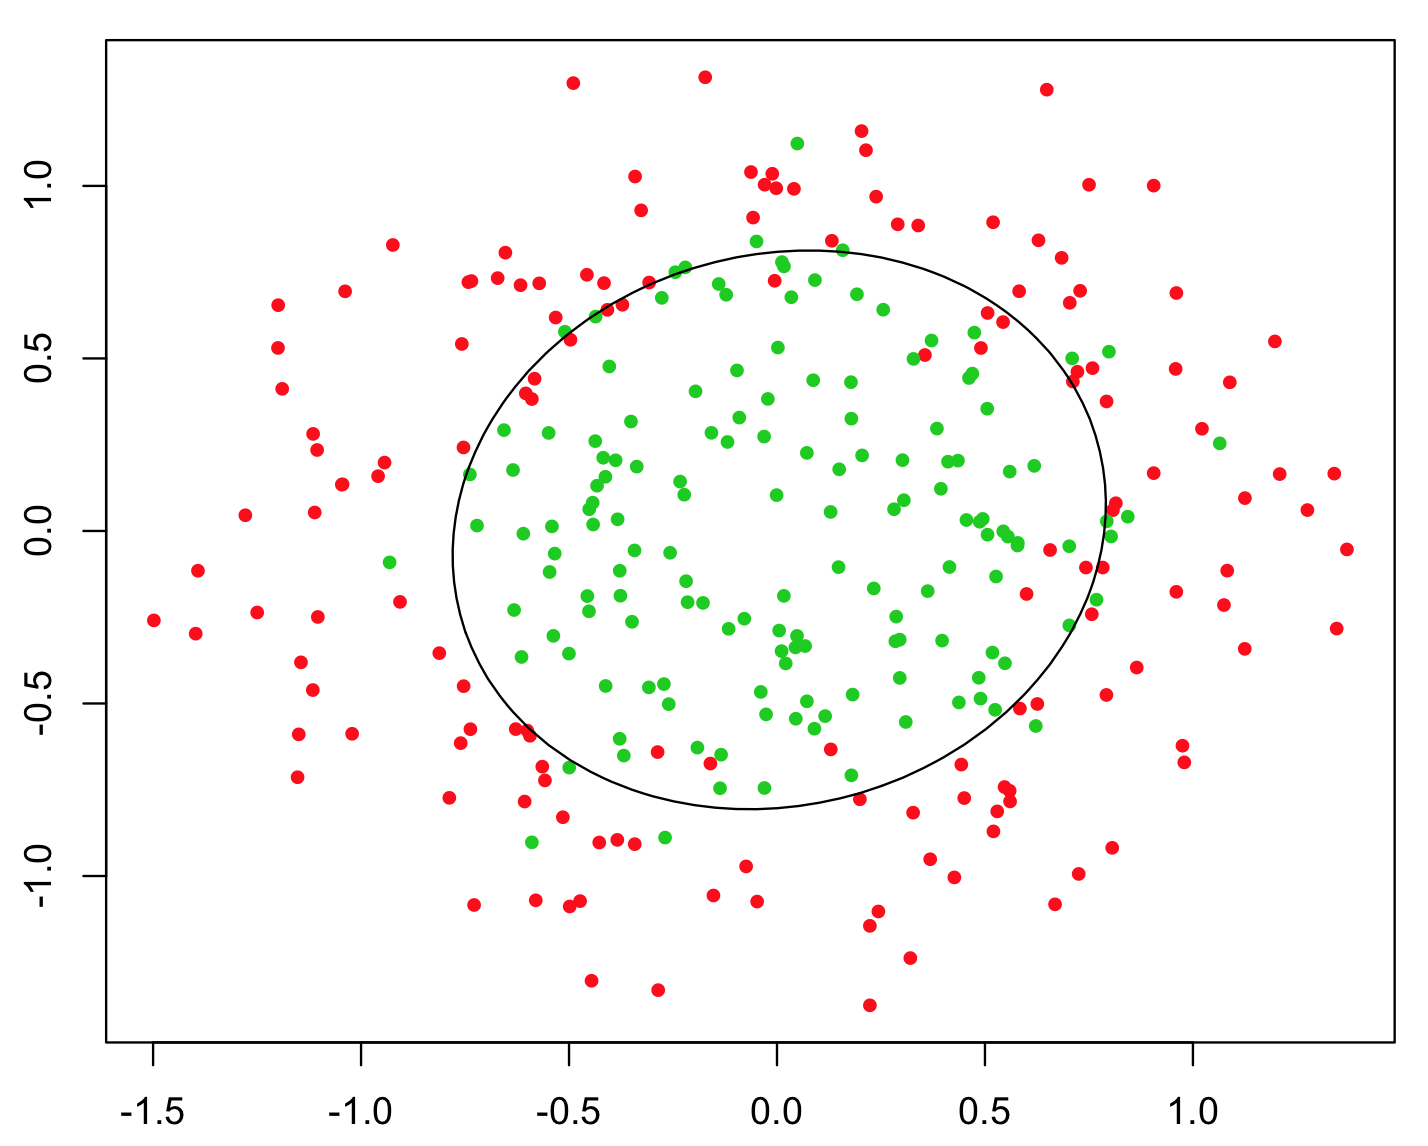
\includegraphics[width=0.4\textwidth]{decision-boundary-2}
	\caption{Cuadratic Decision boundary}
	\label{fig:decision-boundary-2}
	\end{multicols}
\end{figure}



\noindent We can interpret the output of the hypotheses function as:

\begin{align*}
	h_{\theta}(x) \ge 0.5 \to  y = 1 \\
	h_{\theta}(x) < 0.5 \to  y = 0
\end{align*}

\noindent If we observe Figure \ref{fig:sigmoid} we can observe that in order to get $g(z) \ge 0.5$ we need $z$ to be greater than $0$, in other words:

\begin{align*}
	& h_{\theta}(x) = g(\theta^Tx) \ge 0.5 \to  y = 1 \\
	& \text{when } z = \theta^Tx \ge 0
\end{align*}

\noindent Remember:

\begin{align*}
	& z = 0, e^0 = 1 \Rightarrow g(z) = 1/2 \\
	& z \to \infty, e^{\infty} \to 0 \Rightarrow g(z) = 1 \\
	& z \to -\infty, e^{-\infty} \to 0 \Rightarrow g(z) = 0 \\
\end{align*}

\subsection{Cost Function}
We cannot use the same cost function that we use for linear regression because the Logistic Function will cause the output to be wavy, causing many local optima. In other words, it will not be a convex function.

\begin{align*}
	& J(\theta) = \frac{1}{m} \sum_{i=1}^{m}Cost(h_{\theta}(x^{(i)}), y^{(i)}) \\
	& Cost(h_{\theta}(x), y) = -log(h_{\theta}(x)) \qquad\qquad\qquad \text{if } y = 1 \\
	& Cost(h_{\theta}(x), y) = -log(1 - h_{\theta}(x)) \qquad\qquad \text{if } y = 0 \\
\end{align*}

If our correct answer '$y$' is $0$, then the cost function will be $0$ if our hypothesis function also outputs $0$. If our hypothesis approaches $1$, then the cost function will approach infinity.

If our correct answer '$y$' is $1$, then the cost function will be $0$ if our hypothesis function outputs $1$. If our hypothesis approaches $0$, then the cost function will approach infinity.

Note that writing the cost function in this way guarantees that $J(\theta)$ is convex for logistic regression.

\begin{align*}
	& Cost(h_{\theta}(x), y) \to \infty \text{ if } y = 1 \text{and } h_{\theta}(x) \to 1 \\
	& Cost(h_{\theta}(x), y) \to \infty \text{ if } y = 0 \text{and } h_{\theta}(x) \to 0 \\
\end{align*}

\begin{figure}[h]
	\begin{multicols}{2}
	\centering
	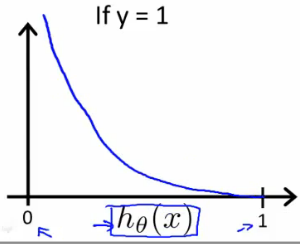
\includegraphics[width=0.4\textwidth]{logistic-regression-cost}
	\caption{$-log(h_{\theta}(x))$}
	\label{fig:logistic-regression-cost}

	\centering
	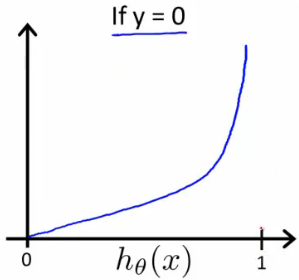
\includegraphics[width=0.4\textwidth]{logistic-regression-cost-2}
	\caption{$-log(1 - h_{\theta}(x))$}
	\label{fig:logistic-regression-cost-2}
	\end{multicols}
\end{figure}

\noindent But there is a much simpler and compat way to represent that conditional:

\begin{align}
	J(\theta) = \frac{1}{m} \sum_{i=1}^{m} -y^{(i)}log(h_{\theta}(x^{(i)})) - (1-y^{(i)})log(1 - h_{\theta}(x^{(i)}))
	\label{logistic-regression}
\end{align}

\noindent And this is the vectorized implementation:

\begin{align}
	J(\theta) = \frac{1}{m} \left(-y^Tlog(g(X\theta)) - (1 - y)^Tlog(1 - g(X\theta)))\right)
\end{align}

\subsection{How to obtain $\theta_{j}$}
The idea, as in linear regression, is to minimize \textbf{Cost Function} (minimize the error). To do that we got many methods:

\begin{enumerate}[label=\textbullet]
	\item \textit{Gradient Descent}
	\item \textit{Conjugate Gradient}
	\item \textit{BFGS}
	\item \textit{L-BFGS}
\end{enumerate}

\noindent In order to use this any of these methods we need our function to return 2 things:

\begin{enumerate}[label=\arabic*.]
	\item \underline{\textit{Value of cost}}: It is just the scalar value of the cost function.
	\item \underline{\textit{Gradient}}: It is the derivative of the cost function ($\frac{\partial{J(\theta)}}{\partial{\theta_j}}$)
\end{enumerate}


\noindent \textbf{Note}: For academic and learning purposes, we are going to only see the Gradient Descent.

\subsubsection{Gradient Descent}
The technique is the same as linear regression, and it has the form:

$$\frac{\partial{J(\theta)}}{\partial{\theta_j}} = \sum^{m}_{i=1}(h_{\theta}(x^{(i)}) - y^{(i)})x^{(i)_j}$$

\begin{flalign*}
	& \text{Repeat} \lbrace  \\
	& \qquad \theta_j := \theta_j - \alpha\frac{\partial{J(\theta)}}{\partial{\theta_j}}  \\
	& \rbrace  
\end{flalign*}

\noindent Notice that this algorithm is identical to the one we used in linear regression. We still have to simultaneously update all values in theta.

\noindent A vectorized implementation is:

$$\theta := \theta - \frac{\alpha}{m}X^T(g(X\theta) - y)$$

\subsection{Multiclass Classification: One-vs-all}

Now we will approach the classification of data when we have more than two categories. Instead of $y = \{0,1\}$ we will expand our definition so that $y = \{0,1 \hdots n\}$.

Since $y = \{0,1 \hdots n\}$, we divide our problem into $n+1$ ($+1$ because the index starts at $0$) binary classification problems; in each one, we predict the probability that '$y$' is a member of one of our classes. The one that has the higher value is the answer.


\begin{align*}
	& y \in \{0,1\hdots n\} \\
	& h_{\theta}^{(0)}(x) = P(y = 0|x;\theta) \\
	& h_{\theta}^{(1)}(x) = P(y = 1|x;\theta) \\
	& h_{\theta}^{(2)}(x) = P(y = 2|x;\theta) \\
	& \vdots \\
	& h_{\theta}^{(n)}(x) = P(y = n|x;\theta) \\
	& \text{prediction } = \max_{i}(h_{\theta}^{(i)}(x))
\end{align*}

\begin{figure}[h]
	\centering
	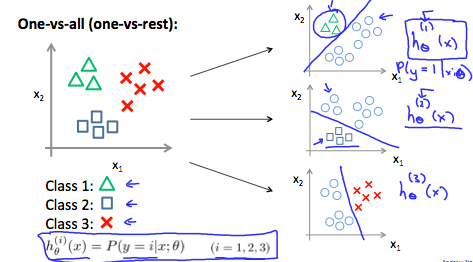
\includegraphics[width=0.7\textwidth]{one-vs-all}
	\caption{One-vs-all multiclass classification}
	\label{fig:one-vs-all}
\end{figure}

\subsection{Underfitting \& Overfitting}
When we are choosing the \textit{Decision Boundary} or the parameters of the \textit{Linear Regression}, and we realize that the function does not fit very well the data. In order to make a better function, we decide to add extra features with different polynomial behaviours; for example, a $5^{th}$ order polynomial.
We observe that even though the fitted curve passes through the data perfectly, we would not expect this to be a good predictor. Now, we got 2 cases: \textbf{underfitting} and \textbf{overfitting}.

\begin{enumerate}[label=\arabic*.]
	\item \textbf{Underfitting}: Also called \textit{high bias}, is when the form of the hypotheses function ($h_{\theta}$) maps poorly to the trend of the data, it means, the function is too simple to predict an accurate value. One reason is because there are very few parameters and cannot generalize very well, thus it cannot make an accurate prediction.
	\item \textbf{Overfitting}: Also called \textit{high variance}, is when the function fits perfectly the available data but does not generalize very well to predict new data. It is usually caused by a complicated function that creates a lot of unnecessary curves and angles unrelated to the data.
\end{enumerate}

There are 2 ways to tackle this issue:
\begin{enumerate}[label=\arabic*.]
	\item \underline{Reduce the number of features}
	\begin{enumerate}[label=\textbullet]
		\item Manually select wich features to keep.
		\item Use model selection algorithm.
	\end{enumerate}
	\item \underline{Regularization}: Keep all the features, but reduces magnitude of parameters $\theta_j$. Works well when we have a lot of slightly useful features.

\end{enumerate}

\subsection{Regularization}
The main goal of regularization is to make the curves less sharp, because we got overfitting problems. In order to do that we gotta reduce the magnitude of $\theta$. As we can see in Figure \ref{fig:regularization}, the function is a more simple with lower curves, which means that now the model can predict with better results by making the parameters to weight more in the cost function (later penalized by the gradient descent algorithm for being too high) and as a result it will reduce it's magnitude.

\begin{figure}[h]
	\centering
	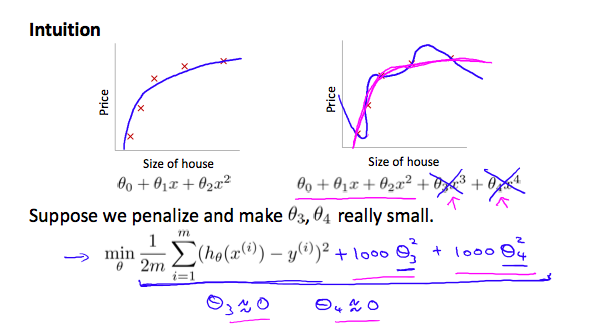
\includegraphics[width=0.7\textwidth]{regularization}
	\caption{Regularization concept}
	\label{fig:regularization}
\end{figure}

To generalize the way to add weight to the parameters ($\theta$), we use a \textbf{regularization parameter} lambda ($\lambda$) multiplied by the sum of the square of the value of the parameters ($\theta$).

$$\frac{\lambda}{2m}\sum^n_{j=1}\theta^2_j$$

Using the cost function with the extra summation above, we can smooth the output of our hypothesis function to reduce overfitting. If lambda is chosen to be too large, it may smooth out the function too much and cause underfitting. If lambda is too small it will cause overfitting as well.

\subsubsection{Regularized Linear Regression}
The form of the regularization for the cost function is: $\frac{\lambda}{2m}\sum^n_{j=1}\theta^2_j$. We \textbf{won't apply regularization on the first parameter (bias)}. So the gradient descent looks like this:

\begin{flalign}
	& \text{Repeat} \lbrace  & \\
	& \qquad \theta_0 := \theta_0 - \alpha
			\frac{1}{m}\sum^m_{i=1}(h_{\theta}(x^{(i)}) - y^{(i)})x^{(i)}_0 & \\
	& \qquad \theta_j := \theta_j - \alpha\Bigg[
		\Bigg( 
			\frac{1}{m}\sum^m_{i=1}(h_{\theta}(x^{(i)}) - y^{(i)})x^{(i)}_j
		\Bigg) + \frac{\lambda}{m}\theta_j
	\Bigg] \qquad\qquad j \in \{1,2\hdots n\} & \\
	& \rbrace  &
\end{flalign}

And the normal equation should look like this (vectorized):

\begin{align*}
	\theta = (X^TX + \lambda \dot L)^{-1}X^Ty \\
	\text{where } L =  \begin{bmatrix}
		0 & & & & \\
		& 1 & & & \\
		& & 1 & & \\
		& & & \ddots & \\
		& & & & 1 \\
	\end{bmatrix}
\end{align*}

\subsubsection{Regularized Logistic Regression}
The form of the regularization for the cost function is: $\frac{\lambda}{2m}\sum^n_{j=1}\theta^2_j$. We \textbf{won't apply regularization on the first parameter (bias)} for this case either. The gradient is the same as the linear.

\noindent When regularization is applied (to solve the overfitting issue), 